\section{Objectives}
\label{chp:objectives}

Given the gap in the academic understanding of the Linux kernel development model when contrasted with the practice, there are undoubtedly several topics that are either not covered at all or investigated in a shallow manner by academic literature. For instance, in the Linux community, there is a quasi-mature discussion about the social challenges, and actions are taken in that regard, like a self-imposed break by Linus Torvalds \cite{linus2018-stepdown} after strong disagreements with the community. There is even a \textit{Code of Conduct} (CoC) \footnote{\href{https://www.kernel.org/doc/html/latest/process/code-of-conduct.html}{Permalink to latest Code of Conduct file}.} that has a committee to handle reported misconduct. Nevertheless, no academic studies covered these topics at all \cite{wen2021-masterthesis}.

Even though social challenges are significant - after all, software engineering considers the process of developing software as a socio-technical phenomenon - this proposed project focuses on understanding the overarching workflows (i.e., the processes and practices) that define the Linux kernel development model.
%
In this sense, we present the two primary objectives of this work:

\begin{itemize}
	\item \textbf{Objective 1}: Validate a theoretical framework that accurately describes the overarching workflows of the Linux kernel development model and allows us to identify bottlenecks;
	\item \textbf{Objective 2}: Develop FLOSS tools that efficiently mitigate bottlenecks in the Linux kernel development model using informed decisions based on a validated theoretical framework.
\end{itemize}

We acknowledge that successfully reaching these objectives does not directly solve all the previously outlined problems. Nonetheless, it does serve as a starting point for ans-wering them.
%
To fulfill these objectives, we will adopt a multi-method approach focusing on \textit{ethographic case-studies} to be close to the practice while also considering the academic literature, grey literature, and community perspectives to triangulate findings and fortify their accuracy.
%
To guide the research, we present three questions:

\begin{enumerate}
    \item \textbf{RQ.1}: What overall workflows compose the Linux kernel development model?
    \item \textbf{RQ.2}: Which processes and/or practices generate bottlenecks in the Linux kernel development model that compromise its efficiency and scalability?
    \item \textbf{RQ.3}: Which bottlenecks can be mitigated by streamlining processes through automation?
\end{enumerate}

\subsection{Expected and preliminary results}

In \textbf{Objective 1}, we aim to validate a taxonomy within the framework of \textit{Grounded Theory} (GT), which involves constructing a structured classification system based on empirical data~\cite{glaser2017-grounded} and its use has become commonplace in the software engineering field~\cite{leite2022-master}. The produced taxonomy will categorize the macro workflows in Linux kernel development, potentially including nested subcategories for finer-grained analysis. Over time, this taxonomy is expected to evolve into an \textit{emergent theory}, a coherent explanatory framework that extends beyond mere classification. This emergent theory will provide a mature and solid foundation for understanding and deriving conclusions about the Linux kernel development model, offering insights into its complexities and workflows.

\begin{figure}[ht]
    \centering
    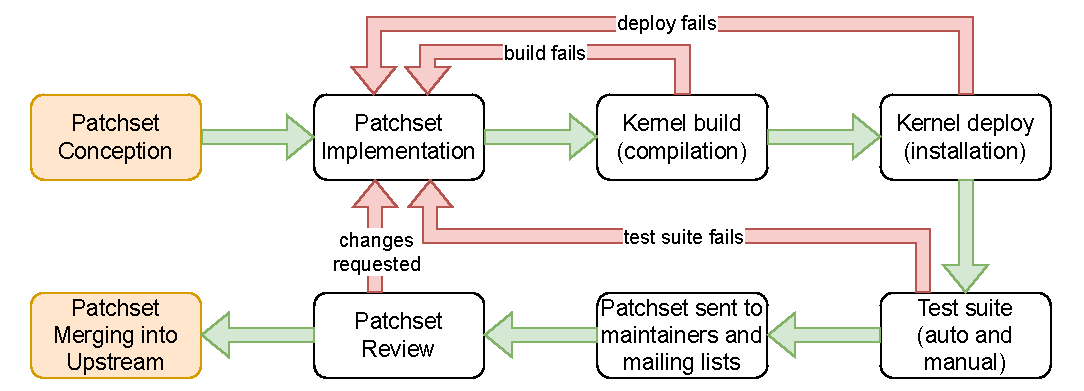
\includegraphics[width=0.8\textwidth]{images/patch-development-workflow.pdf}
    \caption{Concept map of the patchset-development workflow.\label{fig:patch-development-workflow}}
\end{figure}


Figures \ref{fig:patch-development-workflow} and \ref{fig:patchset-reviewing-workflow} illustrate two key workflows in Linux development. Figure \ref{fig:patch-development-workflow} depicts the patchset-development workflow, which spans from the conception of a contribution to its submission, review, and start of merging into the upstream. It includes technical processes like kernel compilation and deployment, as well as practices such as sending patches to the correct maintainers and participating in the review process. Figure \ref{fig:patchset-reviewing-workflow} focuses on the patchset-reviewing workflow, which is more relevant to maintainers. It outlines steps from fetching and selecting patchsets to providing feedback or initiating the merging process. Both workflows highlight the interactive and collaborative nature of Linux development, with variations depending on the subsystem and development context. These concept maps were derived from \textit{Participant Observation}, where the doctoral student: (i) contributed to subsystems like \textit{AMD GPU}, \textit{Industrial I/O}, and \textit{staging}; (ii) developed and maintained tools that support the community; (iii) mentored newcomers into Linux development.

\begin{figure}[ht]
    \centering
    \includegraphics[width=0.6\textwidth]{images/patchset-reviewing-workflow.png}
    \caption{concept map of the patchset-reviewing workflow.\label{fig:patchset-reviewing-workflow}}
\end{figure}


The doctoral student's ongoing development of FLOSS tools to support the Linux ecosystem aligns with \textbf{Objective 2}. By leveraging insights from the taxonomy iterations, informed decisions can be made to address bottlenecks and improve workflows. These tools, such as those aiding patch submission and review, aim to streamline processes and enhance efficiency within the Linux development model. This iterative approach ensures that the tools are grounded in the realities of the Linux ecosystem, addressing actual needs identified through systematic analysis.


